\documentclass[journal]{IEEEtran} % use the `journal` option for ITherm conference style
\IEEEoverridecommandlockouts
% The preceding line is only needed to identify funding in the first footnote. If that is unneeded, please comment it out.
\usepackage{cite}
\usepackage{amsmath,amssymb,amsfonts}
\usepackage{algorithmic}
\usepackage{graphicx}
\usepackage{hyperref}
\usepackage{textcomp}
\usepackage{xcolor}
\usepackage{url}
\graphicspath{ {./figures/} }
\hypersetup{
    colorlinks=true,
    linkcolor=black,
    urlcolor=black,
    citecolor=black
    }

\urlstyle{same}
%\usepackage{draftwatermark}
\def\BibTeX{{\rm B\kern-.05em{\sc i\kern-.025em b}\kern-.08em
    T\kern-.1667em\lower.7ex\hbox{E}\kern-.125emX}}


%\SetWatermarkText{DRAFT} % Watermark text
%\SetWatermarkAngle{45}   % Angle at which watermark appears
%\SetWatermarkLightness{0.93} % Opacity (0 = fully transparent, 1 = fully opaque)
%\SetWatermarkScale{1}    % Watermark scale




\begin{document}

\title{Dataframes Unleashed: Unlocking Effortless Modeling and Performance in Data Analysis with Data Virtual Machines (DVMs)
% delete or comment-out the following line before submission
%{\footnotesize \textsuperscript{*}Note: Sub-titles are not captured in Xplore and should not be used}
\thanks{Identify applicable funding agency here. If none, delete this.}
}

\author{%%%% author names
    \IEEEauthorblockN{1\textsuperscript{st} Given Name Surname}% first author
    , \IEEEauthorblockN{2\textsuperscript{nd} Given Name Surname}% delete this line if not needed
    , \IEEEauthorblockN{3\textsuperscript{rd} Given Name Surname}% delete this line if not needed
    % duplicate the line above as many times as needed to list all authors
    \\%%%% author affiliations
    \IEEEauthorblockA{\textit{dept. name of organization (of Aff.), City, Country}}\\% first affiliation
    \IEEEauthorblockA{\textit{dept. name of organization (of Aff.), City, Country if needed}}\\% delete this line if not needed
    % duplicate the line above as many times as needed to list all affiliations
    %%%% corresponding author contact details
    \IEEEauthorblockA{email address or ORCID of corresponding author(s)}
}

\maketitle

\begin{abstract}

In the era of big data, efficient data analysis is crucial for extracting valuable insights. On the other hand, the diversity of data systems, file formats, and different analysis types including machine learning models introduce challenges for the quick consolidation of the business data in one data model. To address this issue this paper introduces a cutting-edge concept named Data Virtual Machine (DVM) that revolutionizes data analysis with its user-friendly front-end, flexible data modeling, competitive performance, and innovative data virtualization capabilities. Data Virtual Machine (DVM) is a term used to describe an innovative graph-based conceptual model, resembling an entity-relationship model, that represents relationships between different types of data found in organizational and business settings. This model provides individuals, who lack a technical background but are interested in analyzing data for business-related objectives, the ability to define queries leveraging the adaptable schema and the rapid results enabled by the DVM's capabilities to execute calculations on dataframes seamlessly. Traditionally, data analysis tasks are carried out by experienced data analysts that use procedural approaches which have inherent limitations. With DVMs, the data analysis can be performed visually through an intuitive tool, allowing non-IT experts to participate. Various logical data models can be implemented by the DVM and the focus can be dynamically adjusted to different nodes enabling the analysis of data relationships from different perspectives. Furthermore, DVMs implement data virtualization with the support of data sharing, and portability, and provide a unified view of entities, as each DVM node represents both an attribute and an entity. In this study, we present the optimized version of DataMingler that not only offers ease in data analysis but also delivers rapid results in advanced data analysis cases. This optimization is made possible by leveraging concurrency and parallelization in the calculations performed by DataMingler. Through a comprehensive benchmarking study, we demonstrate the tool's remarkable performance compared to traditional Python implementations.

\end{abstract}

\begin{IEEEkeywords}
    Dataframes, Data Analysis, Data Virtualization, Graph Data Model, Data Virtual Machines, Efficient Evaluation, User-Friendly Front-End, Big Data, Modeling, Benchmarking, Python, Data Exploration, Insights, Performance
\end{IEEEkeywords}

\section{Introduction}

Modern analytics environments grapple with the complexity of managing diverse datasets originating from various applications or collected by autonomous agents. Over the last decade, Business Analytics (BA) has evolved significantly through four eras: Analytics 1.0 to Analytics 4.0. In Analytics 1.0, traditional analytical tools were used for decision-making until 2005. The emergence of Big Data marked Analytics 2.0, led by companies like Google and Facebook. Analytics 3.0 combined Big Data and small data analytics for decision support and product creation, while Analytics 4.0, the current era, emphasizes autonomy and democratizing analytics tasks with new job roles like citizen data scientists and business translators alongside quantitative analysts and data scientists \cite{Aleksic2019}. The definition of big data has evolved rapidly, causing confusion among executives due to varying perspectives on its characteristics. The Three V's - Volume, Variety, and Velocity - serve as a common framework to describe big data, representing its high-volume, high-velocity, and high-variety nature. Other dimensions like Veracity, Variability, and Value have also been considered in defining big data. Universal benchmarks do not exist, and the definition depends on factors such as the firm's size, sector, and location. The Three-V tipping point signifies when traditional data management and analysis technologies become inadequate for handling big data efficiently \cite{GANDOMI2015137}. The high-variety datasets exhibit heterogeneity not only in their semantics but also in the data structures that store them and the systems that manage and process them. Utilizing Big Data poses significant challenges for managers across different business functions. To leverage its potential, a new profession, data scientist, with specific skill sets is necessary. This heterogeneity has created the need for different roles in the analytics environment including developers, data engineers, data scientists, data analysts, business users, and data regulation officers, that undertake different analysis projects, ranging from traditional business intelligence to data exploration, data mining, and prediction \cite{Mauro2016}. As of 2016, there was a shortage of approximately 190,000 data scientists in the United States alone \cite{Aleksic2019}.

To effectively address the challenges posed by this diverse landscape, multiple data systems and analysis platforms must coexist, integrated, and federated. While data warehousing has been a common approach, it becomes rigid in rapidly changing data environments. Furthermore, there is a need for techniques that allow the creation of late-bound schemas on data that may be persisted but rarely processed or even never processed. This requirement becomes particularly prevalent in dynamic data infrastructures where analysis objectives change with agility. In such environments, creating comprehensive classical integrated schemas encompassing structured, semi-structured, and unstructured data proves to be not only highly time and resource-intensive but often unattainable within the time constraints of analysis \cite{abadi2016beckman}. As an alternative, many production environments adopt a programming language (e.g., Python, R, Scala) to ad-hoc extract, transform, and assemble data, such as in dataframes, to swiftly build models or reports. Python is a popular open-source programming language supported on various platforms. It offers thousands of third-party packages, including NumPy, Scikit, and Pandas, which are essential for machine learning and data mining tasks. These packages provide support for scientific computing, data preprocessing, modeling, and analysis, making Python user-friendly and suitable for quick problem analysis \cite{Bhadani2016}. Although dataframe libraries in R and Python have achieved considerable success, they encounter performance problems when dealing with moderately large datasets. Additionally, there is considerable uncertainty about the precise meaning or interpretation of dataframe semantics \cite{petersohn2020scalable}. Moreover, this approach lacks data exploration capabilities for end-users, as generating new datasets necessitates creating entirely new programs. 

Python and R offer support for dataframe abstraction, which is a functional interface better suited for developers and data scientists implemented through data science notebooks. Dataframes are more tolerant of unknown data structures and are widely used in data exploration. They possess several characteristics that make them attractive for this purpose: intuitive data model, query language versatility, dataframes offer a query language that bridges various data analysis modes, including relational operations (e.g., filter, join), linear algebra (e.g., transpose), and spreadsheet-like functions (e.g., pivot), incrementally composable query syntax and native embedding in host languages \cite{perez2015project}. Pandas, the library within Python, has been a popular choice for data exploration. However, the rich API of pandas has led to redundancies, making it challenging for users to manually plan queries and optimize performance. The complexity of the API also hinders traditional query optimization techniques. Additionally, pandas' performance breaks down when processing moderate volumes of data that exceed memory limits \cite{petersohn2020scalable}.

As a response to that issue, we propose the following research question.
\textbf{Research question:} \textit{Can a virtual data machine that works on top of the organization data infrastructure as a layer that establishes on-demand connections with the required data sources offer easy dataframe queries formulation by no programming expert users and competitive performance to other traditional python-notebook-based solutions?}

To tackle this challenge, we propose the Data Virtual Machine (DVM), a novel graph-based conceptual model based on entities and attributes, concepts that users intuitively understand. The fundamental idea behind the DVM is both simple and powerful: given a computation C with an output (o1, o2), where o1 belongs to attribute domain A and o2 belongs to attribute domain B, the output of C can be represented as a mapping between A and B. This mapping can be depicted in a graph with nodes A and B and edges representing the mappings as manifested by C's output, which can encompass queries, scripts, programs, and more. The DVM introduces agile and on-demand modeling capabilities, allowing end-users to easily define computations over the data sources, covering relational and non-relational data, streams, and stand-alone programs, visually. As a result, the DVM is automatically generated, reflecting a collection of computations based on their output. This approach diverges from traditional data integration techniques, where the focus is on settling on a fixed schema and then defining data processing tasks to populate or refresh it in data warehousing, or utilizing wrappers to bind data with a virtual schema in case of mediators/virtual databases. Instead, the DVM fits existing data to dynamically constructed schemas, providing greater flexibility and adaptability to evolving analysis requirements. Additionally, it facilitates easy and intuitive querying, enabling non-database experts, such as data scientists and statisticians, to express queries using a high-level query definition language similar to SQL. The DVM's visualization-driven approach effectively hides query optimization and structural details, enhancing usability.

This paper's contributions encompass the introduction of the DVM as a novel conceptual model, a declarative approach to dataframing in analytics environments, and the proposal of an algebraic framework for efficient query evaluation along with concurrency and parallelization optimizations in the calculations. A case study validates the effectiveness of DVMs and the visual DVM query language in effortlessly creating advanced dataframes analysis that would otherwise require programming skills. Moreover, a benchmarking of the DataMigler tool is performed against the traditional Python-notebook-based implementations that demonstrate the superior performance of DataMigler in the query evaluation.

The subsequent sections elaborate on key analytics environment concepts, present the DVM's formal definition and intuitive explanation, introduce DVM dataframe queries and the algebraic framework for their evaluation, discuss query evaluation and optimization, showcase a case study as a proof-of-concept, benchmarking of the tool, and conclude with limitations and future directions for this innovative approach.

\section{Dataframes \& Python}

\subsection{Dataframes History}

Dataframes were initially introduced in the S programming language at Bell Laboratories in 1990 to facilitate statistical computations. The concept of dataframes was presented by Chambers, Hastie, and Pregibon at the Computational Statistics conference. They described dataframes as a class of objects in S that can conveniently organize variables relevant to specific analyses \cite{chambers1990statistical}. Subsequently, Chambers and Hastie expanded on this idea in a book published in 1992 \cite{chambers1992statistical}. In the book, they emphasized that data frames are more flexible than matrices because matrices in S assume all elements to be of the same type, whereas data frames can handle variables of different types. Additionally, data frames enable matrix-like computation with columns as variables and rows as observations and allow computations in which variables are treated separately and accessed by name. The R programming language, which is an open-source implementation of S, was released in 1995 and quickly gained popularity among statisticians. In 2008, Wes McKinney developed pandas, a Python library, aiming to bring dataframe capabilities with R-like semantics to Python, leading to its widespread adoption.\cite{chambers1992statistical}. In 2011 Wes McKinney introduced Pandas, a Python library designed to work with structured data sets, providing rich data structures and tools for data manipulation and analysis. It aims to be a foundational layer for statistical computing in Python and complements the existing scientific Python stack. Pandas address the need for rich data structures and metadata handling through its dataframe object, which allows for flexible and intuitive manipulation of labeled data sets, ensures automatic data alignment, and supports hierarchical indexing for advanced representation of higher-dimensional data within a 2D dataframe \cite{McKinney2011}.


\subsection{Dataframe Data Model}

Chambers and Hastie acknowledge that dataframes are distinct from familiar mathematical objects. Dataframes do not neatly fit into the categories of relations, matrices, or tensors. Instead, they adopt relational terminology from Abiteboul et al. and modify it to suit their purposes \cite{chambers1990statistical}. Dataframes consist of elements from a known set of domains, denoted as \( \text{Dom} = \{\text{dom1, dom2, ...}\} \). For simplicity, the discussion assumes domains are taken from \( \text{Dom} = \{\Sigma^*, \text{int, float, bool, category}\} \), although other domains like date-times are also common in practice. The domain \( \Sigma^* \) represents finite strings over an alphabet \( \Sigma \) and serves as a default, uninterpreted domain (sometimes called Object in certain dataframe libraries). Each domain contains a special null value (NA), and each domain \( \text{domi} \) is associated with a parsing function \( p_i: \Sigma^* \rightarrow \text{domi} \), allowing the interpretation of values in dataframe cells as domain values \cite{abiteboul1995foundations}\cite{petersohn2020scalable}.

A significant feature of dataframes is that the domains of their columns can be induced from data after data acquisition, rather than being declared in advance as in the relational model. They introduce a schema induction function \( S : (\Sigma^*)^m \rightarrow \text{Dom} \) that assigns an array of \( m \) strings to a domain in \( \text{Dom} \). This function is applied to a given column and returns a domain that describes the array of strings in that column. If the domain for any column is not specified, it can be inferred by applying \( S(\cdot) \) to the corresponding column in the data array \( A_{mn} \) \cite{abiteboul1995foundations}\cite{petersohn2020scalable}.

In summary, a dataframe is defined as a tuple \((A_{mn}, R_m, C_n, D_n)\), where \(A_{mn}\) is an array of entries from the domain \(\Sigma^*\), \(R_m\) is a vector of row labels from \(\Sigma^*\), \(C_n\) is a vector of column labels from \(\Sigma^*\), and \(D_n\) is a vector of \(n\) domains from \(\text{Dom}\), one for each column, with the possibility of being left unspecified. The schema of the dataframe is represented by \(D_n\), and if any domain in \(D_n\) is unspecified, it can be induced using the schema induction function \(S(\cdot)\) on the corresponding column of \(A_{mn}\) \cite{abiteboul1995foundations}\cite{petersohn2020scalable}.

Dataframes differ from traditional relational models in the way row and column labels are handled, and they also allow the possibility of defining schemas on rows as well as columns, providing unique cell interpretations and flexibility of interpretation in the algebra. When the schema \(D_n\) has the same domain \(dom\) for all \(n\) columns, they call it a homogeneous dataframe. A special case is the matrix dataframe, which adheres to the properties of a matrix, including support for linear algebra operations when it contains numeric values and operators such as \(+\) and \(\times\) forming a field. Overall, dataframes have elements from both relational and matrix viewpoints, but they are not equivalent to tables or matrices, showcasing unique characteristics and capabilities. The authors intend to use these perspectives to define both relational and linear algebra operations in their dataframe algebra for modern data science work \cite{abiteboul1995foundations}\cite{petersohn2020scalable}.

\subsection{Dataframe Limitations}

Dataframes can be mostly found in the popular Python library named Pandas. Although pandas is praised for its extensive API, it also contains significant redundancies among its operators, leading to varied performance implications. This complexity places a burden on users who need to manually plan queries by selecting the appropriate pandas API calls. For instance, a single task can be achieved using multiple different methods, with performance ranging from very fast to considerably slow. The panda's documentation itself provides several recommendations to improve performance. Consequently, many users opt to use only a small subset of operators, avoiding the bulk of the API. The intricacies of the API and its evaluation semantics make it challenging to apply traditional query optimization techniques. Each operator within a pandas "query plan" is executed entirely before subsequent operators, lacking extensive optimization, reordering, or pipelining, unless explicitly instructed by the user using .pipe. Furthermore, when dealing with even moderately large datasets that exceed memory capacity, the performance of the pandas.DataFrame API declines significantly. This is due to pandas' eager evaluation approach, where intermediate data sizes often surpass memory limits and require paging \cite{petersohn2020scalable}. Regarding memory usage and handling large datasets, pandas is currently limited to in-memory data sets. However, there is a desire to enhance its capabilities to accommodate data sets that surpass memory limits. One approach under consideration involves enabling pandas to seamlessly utilize the multiprocessing module or a parallel computing backend to facilitate large-scale computations without burdening the user with the complexities of managing memory constraints \cite{McKinney2011}.

Moreover, Pandas has several limitations that can impact its effectiveness in handling large datasets. One major concern is its memory usage, as it stores the entire dataset in memory, causing issues with datasets that exceed available memory and leading to performance bottlenecks. Pandas' memory usage is a widely recognized drawback attributed to its internal memory requirements. As suggested by McKinney, the creator of Pandas, it is advisable to have 5 to 10 times more RAM than the dataset's size to mitigate this issue \cite{sinthong2019aframe}. Additionally, complex operations like group by and join can be slow on large DataFrames, although some performance improvements can be achieved with vectorized operations, Cython, or Numba. Nonetheless, other libraries like Dask or Vaex are better suited for efficiently handling larger datasets. Another drawback is Pandas' lack of native support for parallel or distributed computing, which makes it less suitable for large-scale data processing tasks. Although libraries like Dask and Modin extend Pandas' functionality for parallel and distributed computing, they may have their own limitations. As a result, users dealing with larger datasets or working in distributed environments may find alternative libraries like Dask, Vaex, or Apache Spark more appropriate, offering improved performance and scalability for their data processing needs \cite{nelluri2021limitations}. The mentioned alternative libraries, such as Dask, Vaex, and Apache Spark, may present increased complexity and demand advanced programming skills and hardware setup, including cloud infrastructure. Unlike the relatively straightforward usage of Pandas, these libraries have steeper learning curves due to their distributed computing capabilities and specialized features. Working with Dask, Vaex, or Apache Spark may require a deeper understanding of distributed computing concepts, parallel processing, and data shuffling, making them more suitable for experienced data engineers and advanced programmers. Additionally, users may need to set up and configure cloud-based infrastructure to distribute workloads and process data in parallel across multiple nodes or virtual machines.

Some additional general drawbacks of the programming language approach like Python include the following. One of the drawbacks is that end-users who are not proficient in programming may find it challenging to explore data directly, as they would with graphical data exploration tools. Moreover, the lack of reusability in the approach can lead to duplication of effort and maintenance challenges when creating new datasets or performing different analyses. When data sources undergo changes or new data sources are introduced, it becomes challenging to update the code efficiently to accommodate these modifications. This difficulty arises due to the need for manual intervention and adjustments in the existing codebase, which can be time-consuming and error-prone. As data structures and formats evolve, the code must be adapted to handle these alterations, and when new data sources are integrated, the codebase may require significant reworking or rewriting. Additionally, maintaining and updating multiple instances of non-standardized code can become complex and error-prone, making it harder to ensure consistent data processing across the organization. This lack of reusability can hinder collaboration, scalability, and overall efficiency in data-driven projects. 

\subsection{Dataframes expression over DVM} % Old Data Mingler section

DataMingler is a prototype GUI tool to (a) define and manage DVMs, (b) express dataframe queries in a visual and intuitive way, and (c) materialize the DVM (or parts of it) in other logical models – currently only JSON is supported. Data Canvas is the module that enables the creation and manipulation of a DVM by mapping data and processes onto the graph and extending it with new nodes and edges. The data source types that DataMingler currently handles are: relational databases, csv files, excel and stand-alone programs (Java and Python). A DVM is kept in a Neo4j graph database. Dataframe queries can be formulated either textually or visually, using the Query Builder module. In both cases, queries are represented in an XML-based intermediate representation and then parsed and transformed to a key-listalgebraic expression, which is given to the optimizer and an execution plan is generated. Redis is used as the key-value engine for manipulating key-list structures. The JSON Exports module can be used to instantiate model specific databases (currently, JSON is supported). The user selects a node and a breadth-first-search tree rooted on this node is defined. Then the system generates collection of JSON documents corresponding to this tree\cite{chatziantoniou}.

\subsection{Dataframe query operators}

To evaluate a dataframe query such as the one shown in Figure \ref{query1}, some algebraic operators need to be defined. These operators take as input one or more edges is a key-list structure and produce as output a single edge. We can see some of these operators in Definitions 3.3, 3.4, 3.5, 3.6 and 3.7\cite{chatziantoniou}. An in-depth look and analysis of these operators can be seen in the work by Chatzianotniou et. al. (2022)\cite{chatziantoniou}

\textit{Definition 3.3:} \textbf{[Aggregation]} We define an operator called \textit{aggregation}, which gets a key-list structure \(K\) and an aggregate function \(f\) and returns a new key-list structure \(K^'\) constructed as follows: \(\forall k \in keys(K)\), it adds pair \((k, L_k^')\) to \(K^'\), where \(L_k^{'} = [f(L_k)]\), i.e. a list with a single element, the result of the reduced list \(L_k\) according to \(f\). We denote this operator as \(Aggr(K, f)\)\cite{chatziantoniou}. An example of an aggregated function can be the min, max, average, sum or count functions written in any programming language.

\textit{Definition 3.4:} \textbf{[Filtering]} We define an operator called \textit{filtering}, which gets a key-list structure \(K\) and a condition \(\theta\) defined on a single element of a list (a string) and returns a new key-list structure \(K^'\) constructed as follows: \(\forall k \in keys(K)\), it adds to \(K^'\) a pair \((k, L_k^{'})\), where \(L_k^'\) contains all \(x \in L_k\) such that \(\theta(x)\) is true. We denote this operator as \(Filter(K, \theta)\)\cite{chatziantoniou}.

\textit{Definition 3.5:} \textbf{[Mapping]} we define an operator, called \textit{mapping}, which gets as key-list structure \(K\) and a function \(f\) with a signature \texttt{string f(x:string)} and returns a new key-list structure \(K^'\) constructed as follows: \(\forall k \in keys(K)\), it adds to \(K^'\) a pair \((k, L_k^{'})\), where \(L_k^{'} = [f(x): x \in L_k]\), i.e. each element \(x\) in \(L_k\) is replaced by \(f(x)\). We denote this operator as \(Map(K, f)\)\cite{chatziantoniou}. An example of a mapping can be the transformation of customer reviews to sentiment scores using sentiment analysis.

\textit{Definition 3.6:} \textbf{[RollupJoin]} We define an operator, called \textit{RollupJoin}, which gets two key-list structures \(K_1\) and \(K_2\) and returns a new key-list structure \(K\) constructed as follows: \(\forall k \in keys(K_1)\), it adds to \(K\) a pair \((k, L_k)\), where \(L_k = \oplus_{x \in list(k, K_1)}list(x, K_2)\), \(\oplus\) stands for list concatenation. We denote this operator as \(rollUpJoin(K_1, K_2)\)\cite{chatziantoniou}.

\textit{Definition 3.7:} \textbf{[ThetaCombine]} Given:
    \begin{itemize}
        \item a list \(O\) of key-list structures \(K_1, K_2, ..., K_n\), called the \textit{output} list (can be empty)
        \item a list \(S\) of key-list structures \(K_1^{'}, K_2^{'}, ..., K_m^{'}\), called the \textit{selection} list (can be empty)
        \item a boolean expression \(\theta(k, l_1, l_2, ..., l_m)\) involving \(k\) (an atomic value), \(l_1, l_2, ..., l_m\) (lists of values), called the \textit{selection condition}
    \end{itemize}
we define an operator called \textit{ThetaCombine}, denoted as \(thetaCombine(O; S; \theta)\), which returns a key-list structure \(K\) constructed as follows:
\begin{itemize}
\item[] \(\forall k \in keys(K_1)\cap...\cap keys(K_n)\cap keys(K_1^{'}) \cap...\cap keys(K_m^{'})\):

   \quad if \((\theta (k, list(k, K_1^{'}), ..., list(k, K_m^{'})))\) is true:
        
        \quad \quad add a pair \((k, L_k)\) to \(K\), where:
            
            \quad \quad \quad if \(O\) is empty then \(L_k = []\) (the empty list)
            
            \quad \quad \quad else \(L_k = \oplus_{i = 1, 2, ..., n}list(k, K_i)\)\cite{chatziantoniou}
\end{itemize}




\section{Query evaluation \& optimization}

To test the performance of the DataMingler tool we created a set of queries whose execution time was both tested using the tool and traditional data analysis techniques. In particular, we created Jupyter Notebooks that performed the queries using the Python Pandas library and compared the execution time against the DataMingler tool. It is worth noting that apart from performance, the DataMingler tool should be looked at under the scope of ease-of-use and the need for less technical skills to perform queries on multiple data sources. The creation of these notebooks and management of such different data sources is a highly technical and time consuming task. Having a tool that can accelerate the process without any technical knowledge offers many benefits and can save valuable time and resources.

\textbf{Query 1} For each day of the week we want to have the average, minimum, maximum, count and sum of the \texttt{airportFee, driverPay, tripTime, tripMiles, passengerFare} and \texttt{driverTip}. Also we would like to map the \texttt{passengerReviews} to a sentiment score using a sentiment analysis tool to also show the average, minimum, maximum, count and sum of the reviews for each day of the week. A graphical representation of this dataframe query on DVM can be seen in Figure \ref{queryExp1}.

\begin{center}
    \begin{figure}[h]
        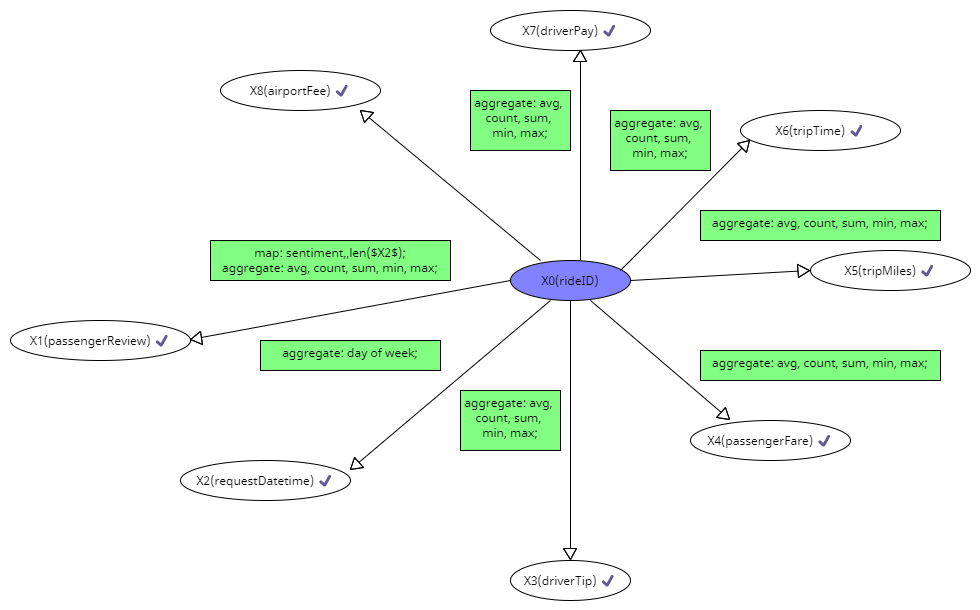
\includegraphics[scale=0.25]{queryExp1}
        \caption{First query of experiment.}
        \label{queryExp1}
    \end{figure}
\end{center}

\textbf{Query 2} For each driver, represented by a unique \texttt{driverUID}, show their \texttt{vehicleModel} and \texttt{gender} along with the average, minimum, maximum, count and sum of their trips \texttt{driverPay, airportFee, passengerReview, driverTip, passengerFare, tripMiles} 
 and \texttt{tripTime}. For the \texttt{passengerReview} the attribute is first going to be mapped using a sentiment analysis tool and then aggregated. A graphical representation of this query on DVM can be seen in Figure \ref{queryExp2}.

\begin{center}
    \begin{figure}[h]
        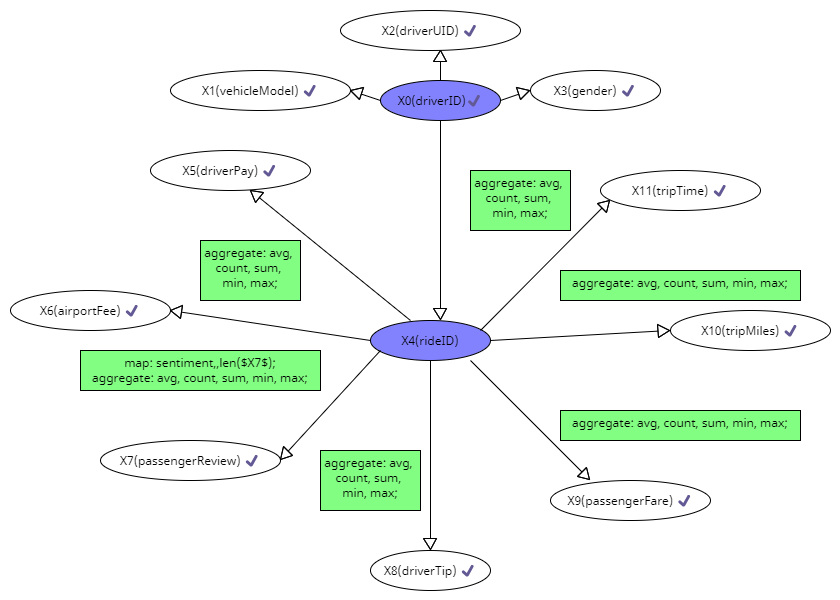
\includegraphics[scale=0.25]{queryExp2}
        \caption{Second query of experiment.}
        \label{queryExp2}
    \end{figure}
\end{center}

\textbf{Query 3} For every location and datetime that taxi trips occurred, represented by \texttt{locationDatetimeID}, show the minimum, maximum, count and sum of the \texttt{airportFee, passengerReview, driverTip, driverPay, passengerFare, tripMiles} and \texttt{tripTime} along with their \texttt{meanCongestion} and \texttt{meanSpeed}. For the \texttt{passengerReview} the attribute is first going to be mapped using a sentiment analysis tool and then aggregated. A graphical representation of this query on DVM can be seen in Figure \ref{queryExp3}.

\begin{center}
    \begin{figure}[h]
        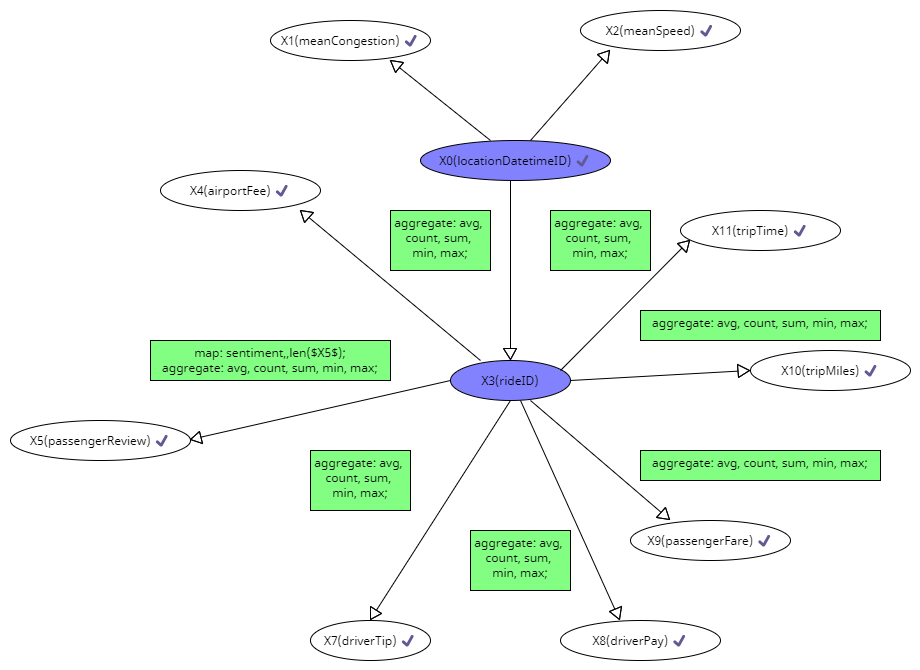
\includegraphics[scale=0.25]{queryExp3}
        \caption{Third query of experiment.}
        \label{queryExp3}
    \end{figure}
\end{center}

\subsection{Algebric evaluation}

\subsection{Optimization}

\newpage
\section{Related Work}

\input{Sections/4.Related Work}

\begin{thebibliography}{00}            
    \bibitem{Aleksic2019}
    Jasna Soldic Aleksic, Biljana Chroneos Krasavac, and Ema Karamata,
    \emph{Business analytics: new concepts and trends},
    \emph{Management: Journal of Sustainable Business and Management Solutions in Emerging Economies}, 
    vol. 25, 
    July 2019,
    doi: \url{10.7595/management.fon.2019.0013}.
    \bibitem{GANDOMI2015137}
    Amir Gandomi and Murtaza Haider,
    \emph{Beyond the hype: Big data concepts, methods, and analytics},
    \emph{International Journal of Information Management}, 
    vol. 35, 
    no. 2, 
    pp. 137-144, 
    2015,
    ISSN 0268-4012,
    doi: \url{https://doi.org/10.1016/j.ijinfomgt.2014.10.007}
    \bibitem{Mauro2016}
    Andrea De Mauro, Marco Greco, Michele Grimaldi, and Giacomo Nobili,
    \emph{Beyond Data Scientists: a Review of Big Data Skills and Job Families},
    in \emph{Proceedings of the Conference Name}, % Replace "Conference Name" with the actual conference name if available
    June 2016.
    \bibitem{Bhadani2016}
    A. Bhadani and D. Jothimani,
    \emph{Big data: Challenges, opportunities and realities},
    In M.K. Singh and D.G. Kumar (Eds.),
    \emph{Effective Big Data Management and Opportunities for Implementation},
    pp. 1-24,
    Pennsylvania, USA,
    IGI Global,
    2016.
    \bibitem{petersohn2020scalable}
    Devin Petersohn, Stephen Macke, Doris Xin, William Ma, Doris Lee, Xiangxi Mo, Joseph E. Gonzalez, Joseph M. Hellerstein, Anthony D. Joseph, and Aditya Parameswaran,
    \emph{Towards Scalable Dataframe Systems},
    \emph{arXiv preprint},
    eprint: 2001.00888,
    archivePrefix: arXiv,
    primaryClass: cs.DB,
    2020.    
    \bibitem{perez2015project}
    Fernando Perez and Brian E. Granger,
    \emph{Project Jupyter: Computational narratives as the engine of collaborative data science},
    Retrieved September, 11(207):108,
    2015.
    \bibitem{abadi2016beckman}
    D. Abadi and others,
    \emph{The Beckman Report on Database Research},
    \emph{Communications of the ACM},
    vol. 59,
    pp. 692–99,
    February 2016.
    \bibitem{chambers1992statistical}
    M. Chambers, T. J. Hastie, and others,
    \emph{Statistical Models in S},
    volume 251,
    Wadsworth \& Brooks/Cole Advanced Books \& Software,
    Pacific Grove, CA,
    1992.
    \bibitem{chambers1990statistical}
    J. Chambers, T. Hastie, and D. Pregibon,
    \emph{Statistical Models in S},
    In K. Momirović and V. Mildner, editors,
    \emph{Compstat},
    pages 317–321,
    Heidelberg,
    1990,
    Physica-Verlag HD.
    \bibitem{McKinney2011}
    Wes McKinney,
    \emph{pandas: a Foundational Python Library for Data Analysis and Statistics},
    \emph{Python High Performance Science Computer},
    January 2011.
    \bibitem{abiteboul1995foundations}
    S. Abiteboul, R. Hull, and V. Vianu,
    \emph{Foundations of Databases},
    volume 8,
    Addison-Wesley,
    Reading,
    1995.
    \bibitem{nelluri2021limitations}
    Ramesh Nelluri,
    \emph{What are the limitations of pandas?},
    \emph{Insights and Data},
    Published on April 10, 2021,
    Available at: \url{https://insightsndata.com/what-are-the-limitations-of-pandas-35d462990c43}.
    \bibitem{sinthong2019aframe}
    Phanwadee Sinthong and Michael J. Carey,
    \emph{AFrame: Extending DataFrames for Large-Scale Modern Data Analysis (Extended Version)},
    \emph{arXiv preprint},
    eprint: 1908.06719,
    archivePrefix: arXiv,
    primaryClass: cs.DB,
    2019.
    \bibitem{chatziantoniou}
    D. Chatziantoniou, V. Kantere, N. Antoniou, A. Gatzia,
    \emph{Data Virtual Machines: Simplifying Data Sharing,
    Exploration \& Querying in Big Data Environments},
    IEEE International Conference on Big Data (Big Data),
    2022.
    
\end{thebibliography}




\end{document}
